\section{Results}
\begin{figure}[ht!]
\centering
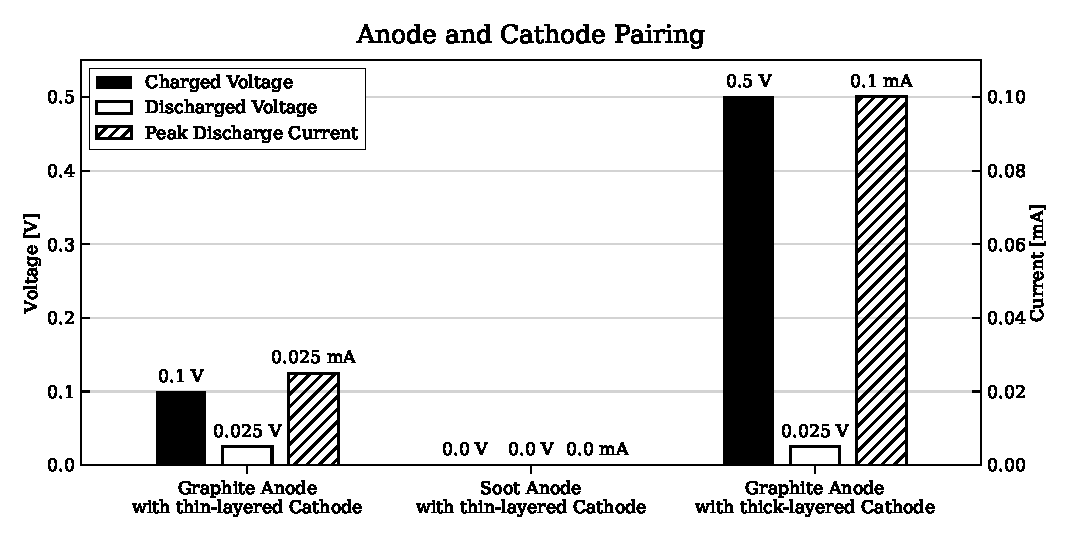
\includegraphics[width=\textwidth]{images/batteryfig.eps}
\caption{The charged and discharged voltage, as well as the peak discharge current of different anode and cathode pairings.}
\label{fig:anodecathodepairing}
\end{figure}

\begin{figure}[ht!]
\centering
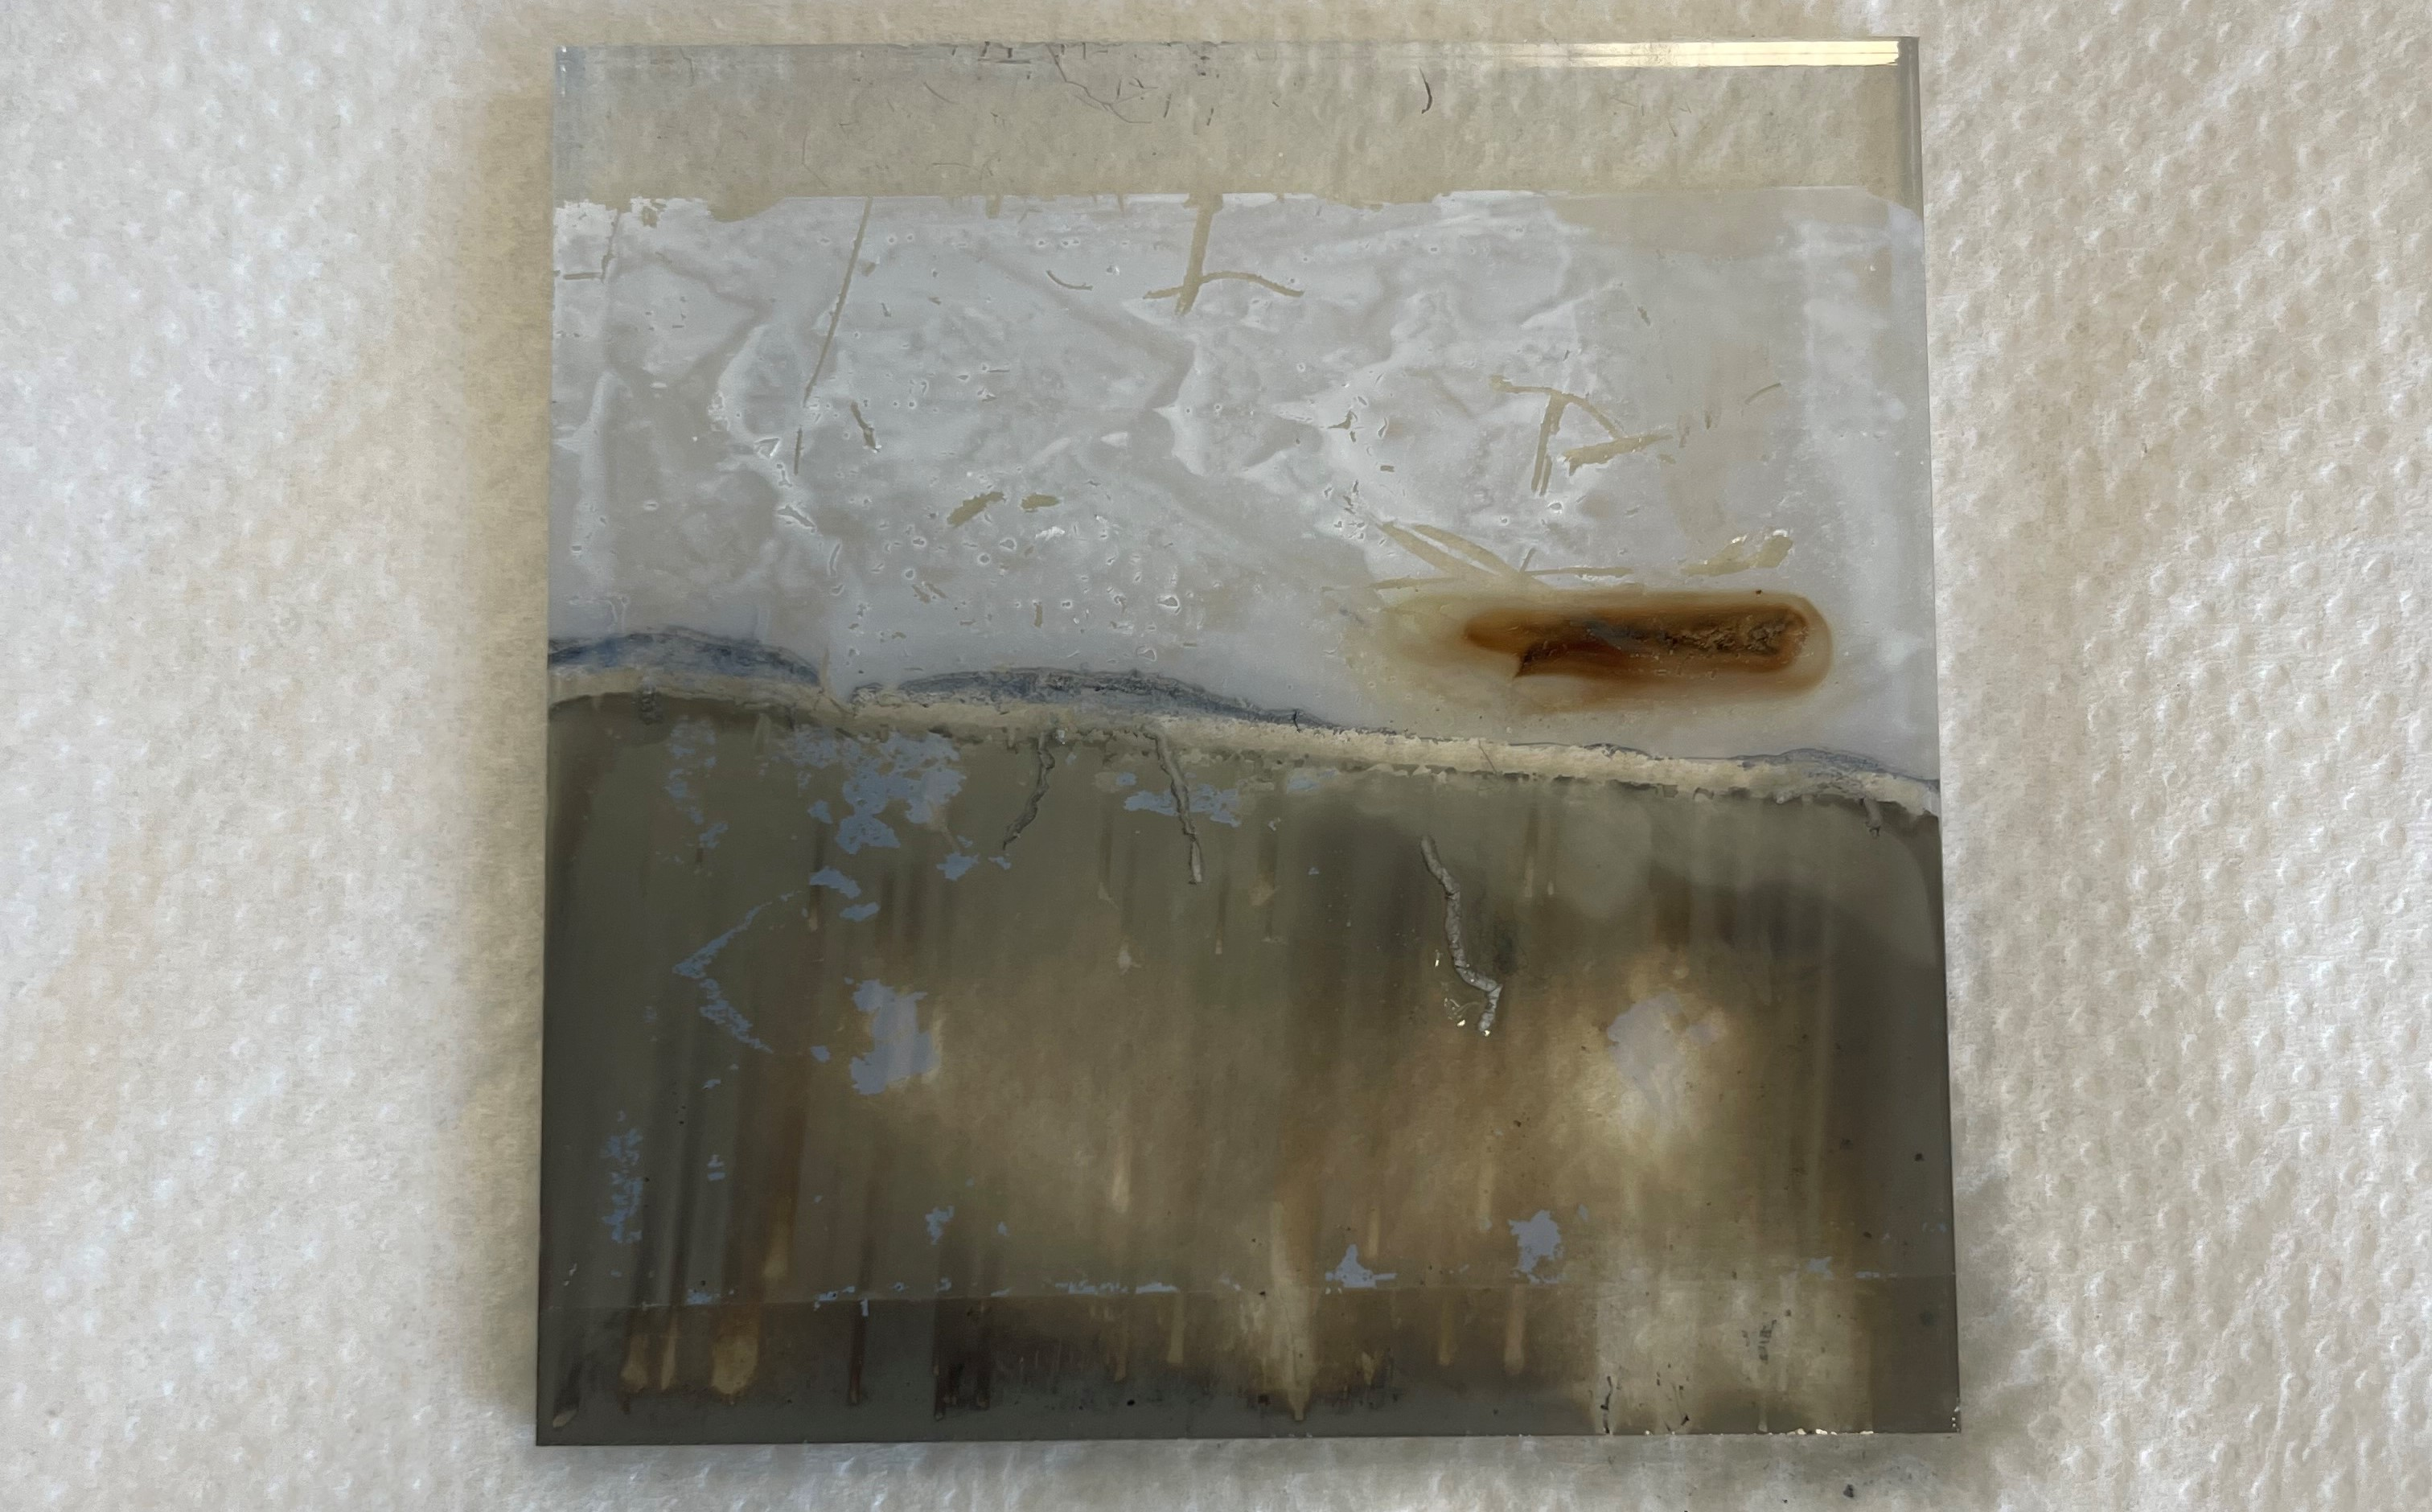
\includegraphics[width=0.9\textwidth]{broken_cathode}
\caption{The cathode permanently damaged by the electrolysis of water.}
\label{fig:brokencathode}
\end{figure}

\begin{figure}[ht!]
\centering
\subfloat[]{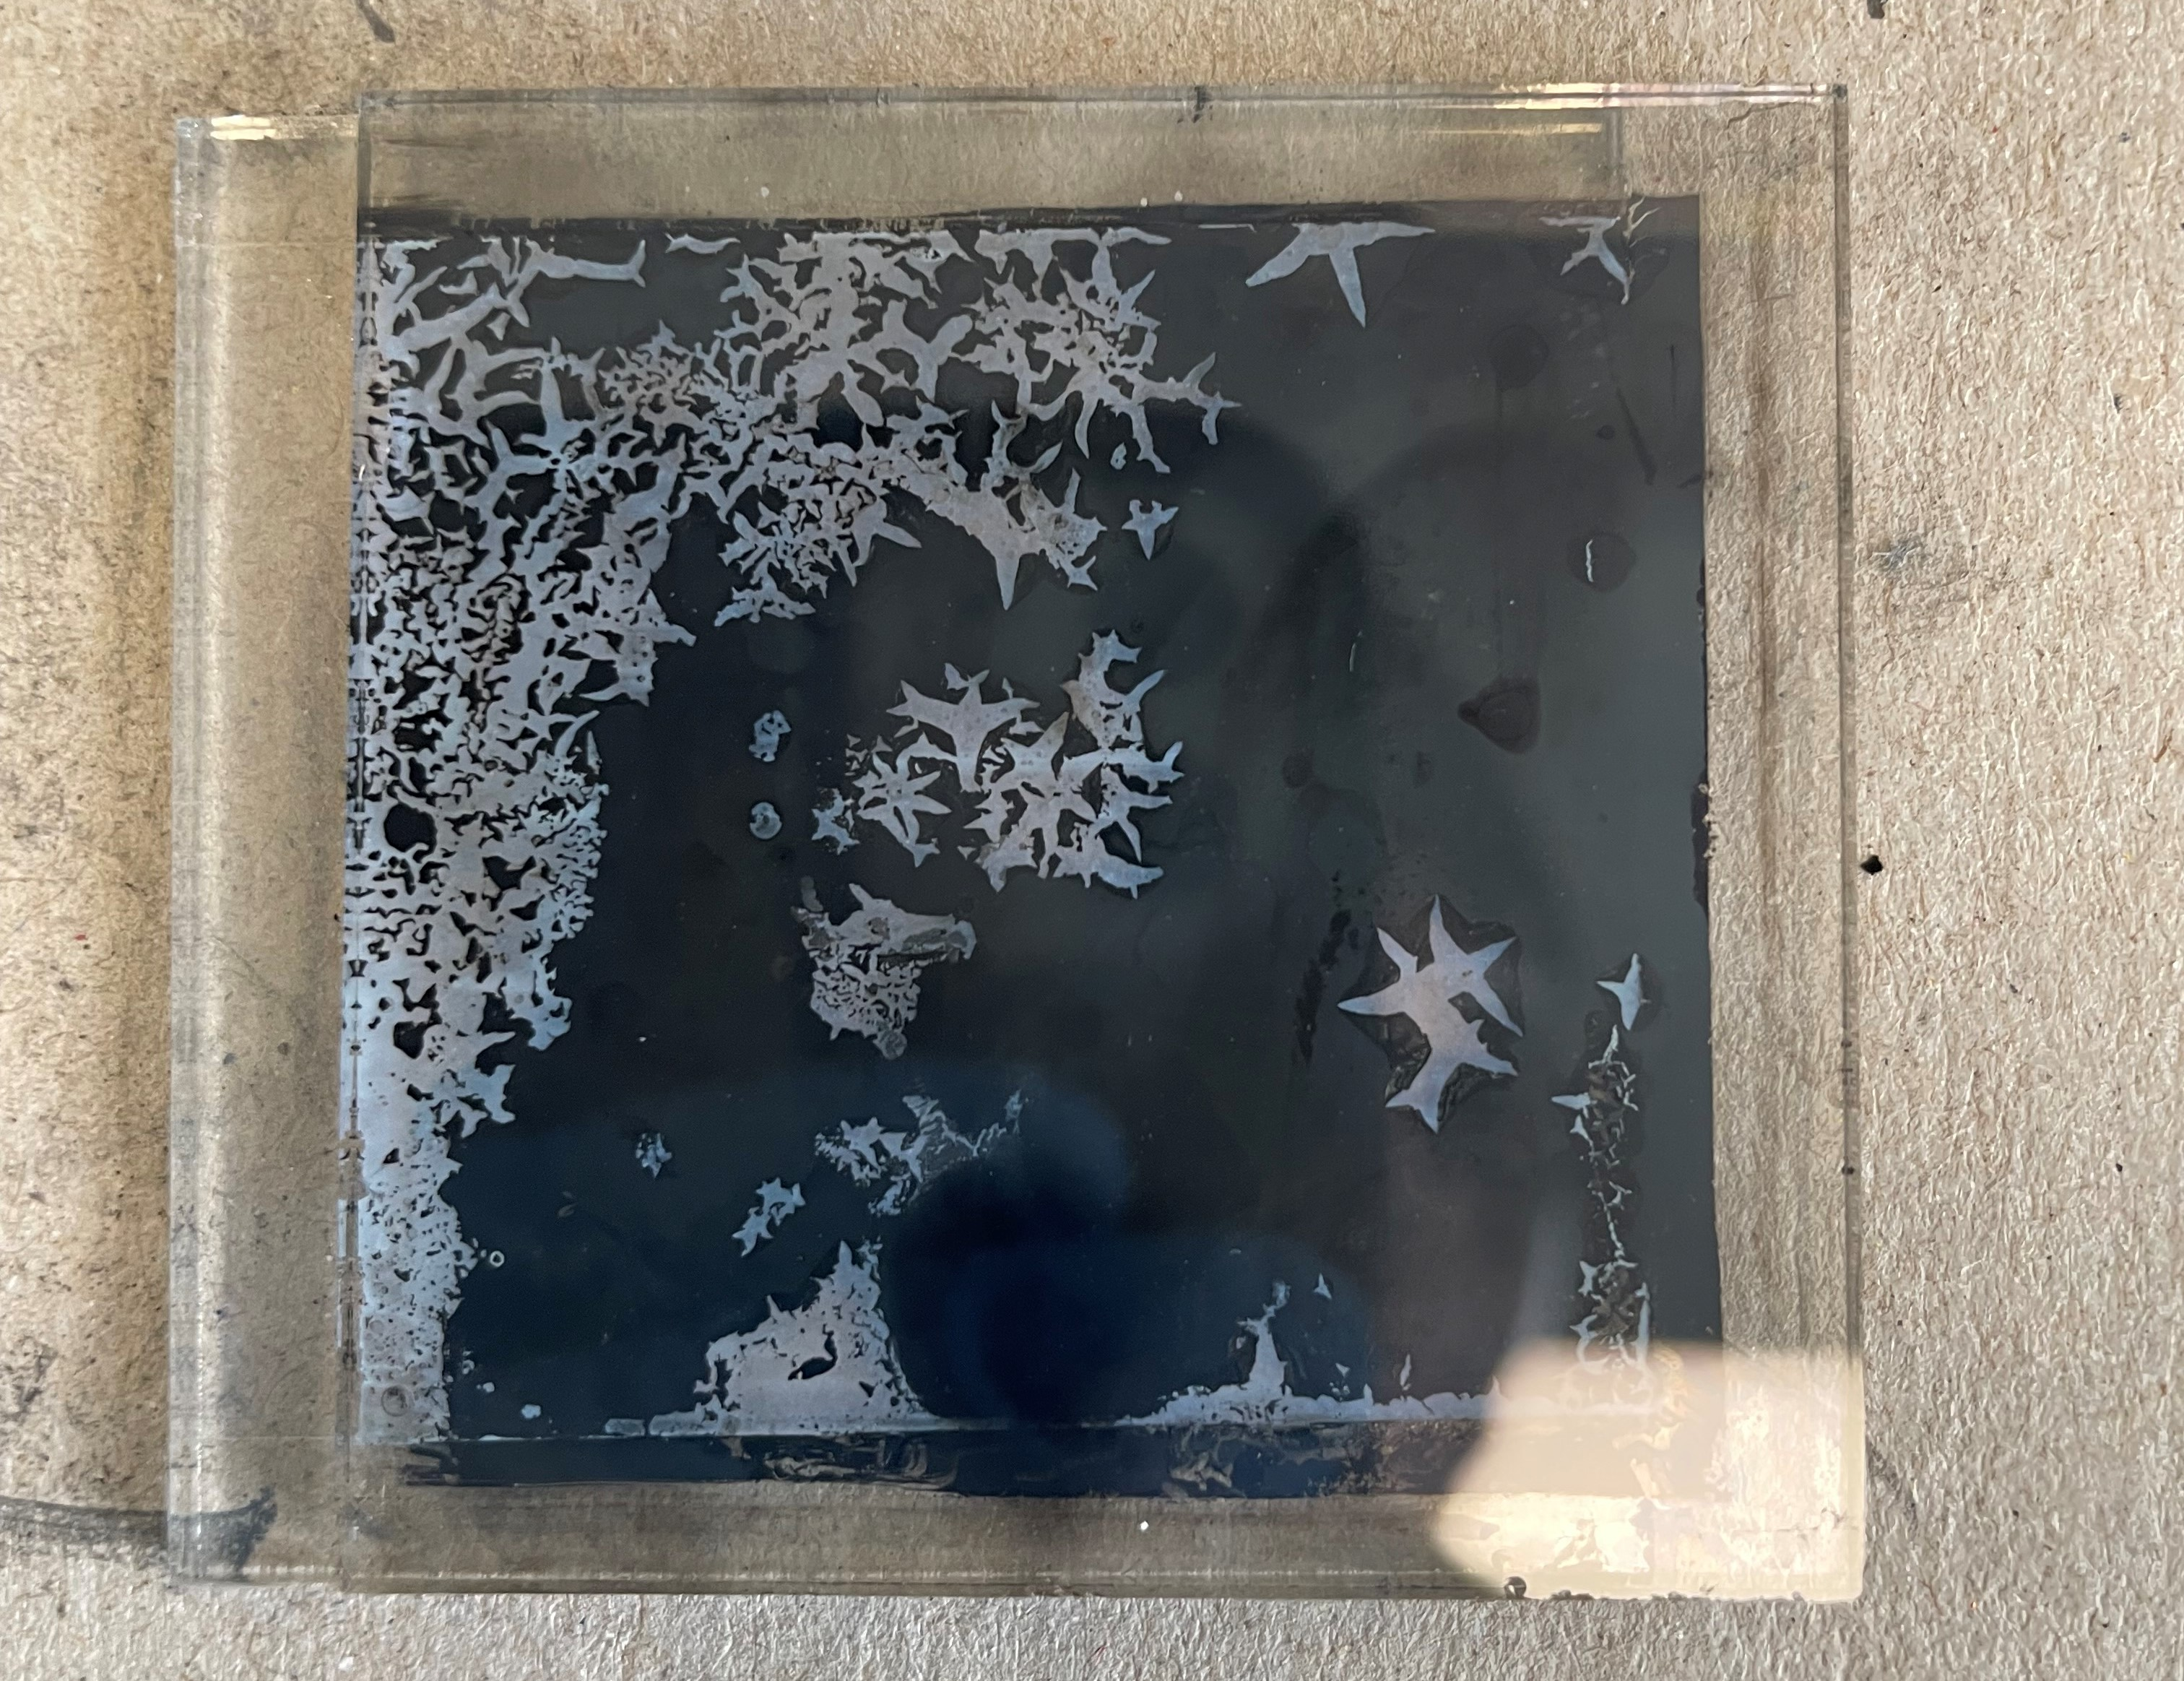
\includegraphics[width=0.256\textwidth]{broken_soot_anode}}
\subfloat[]{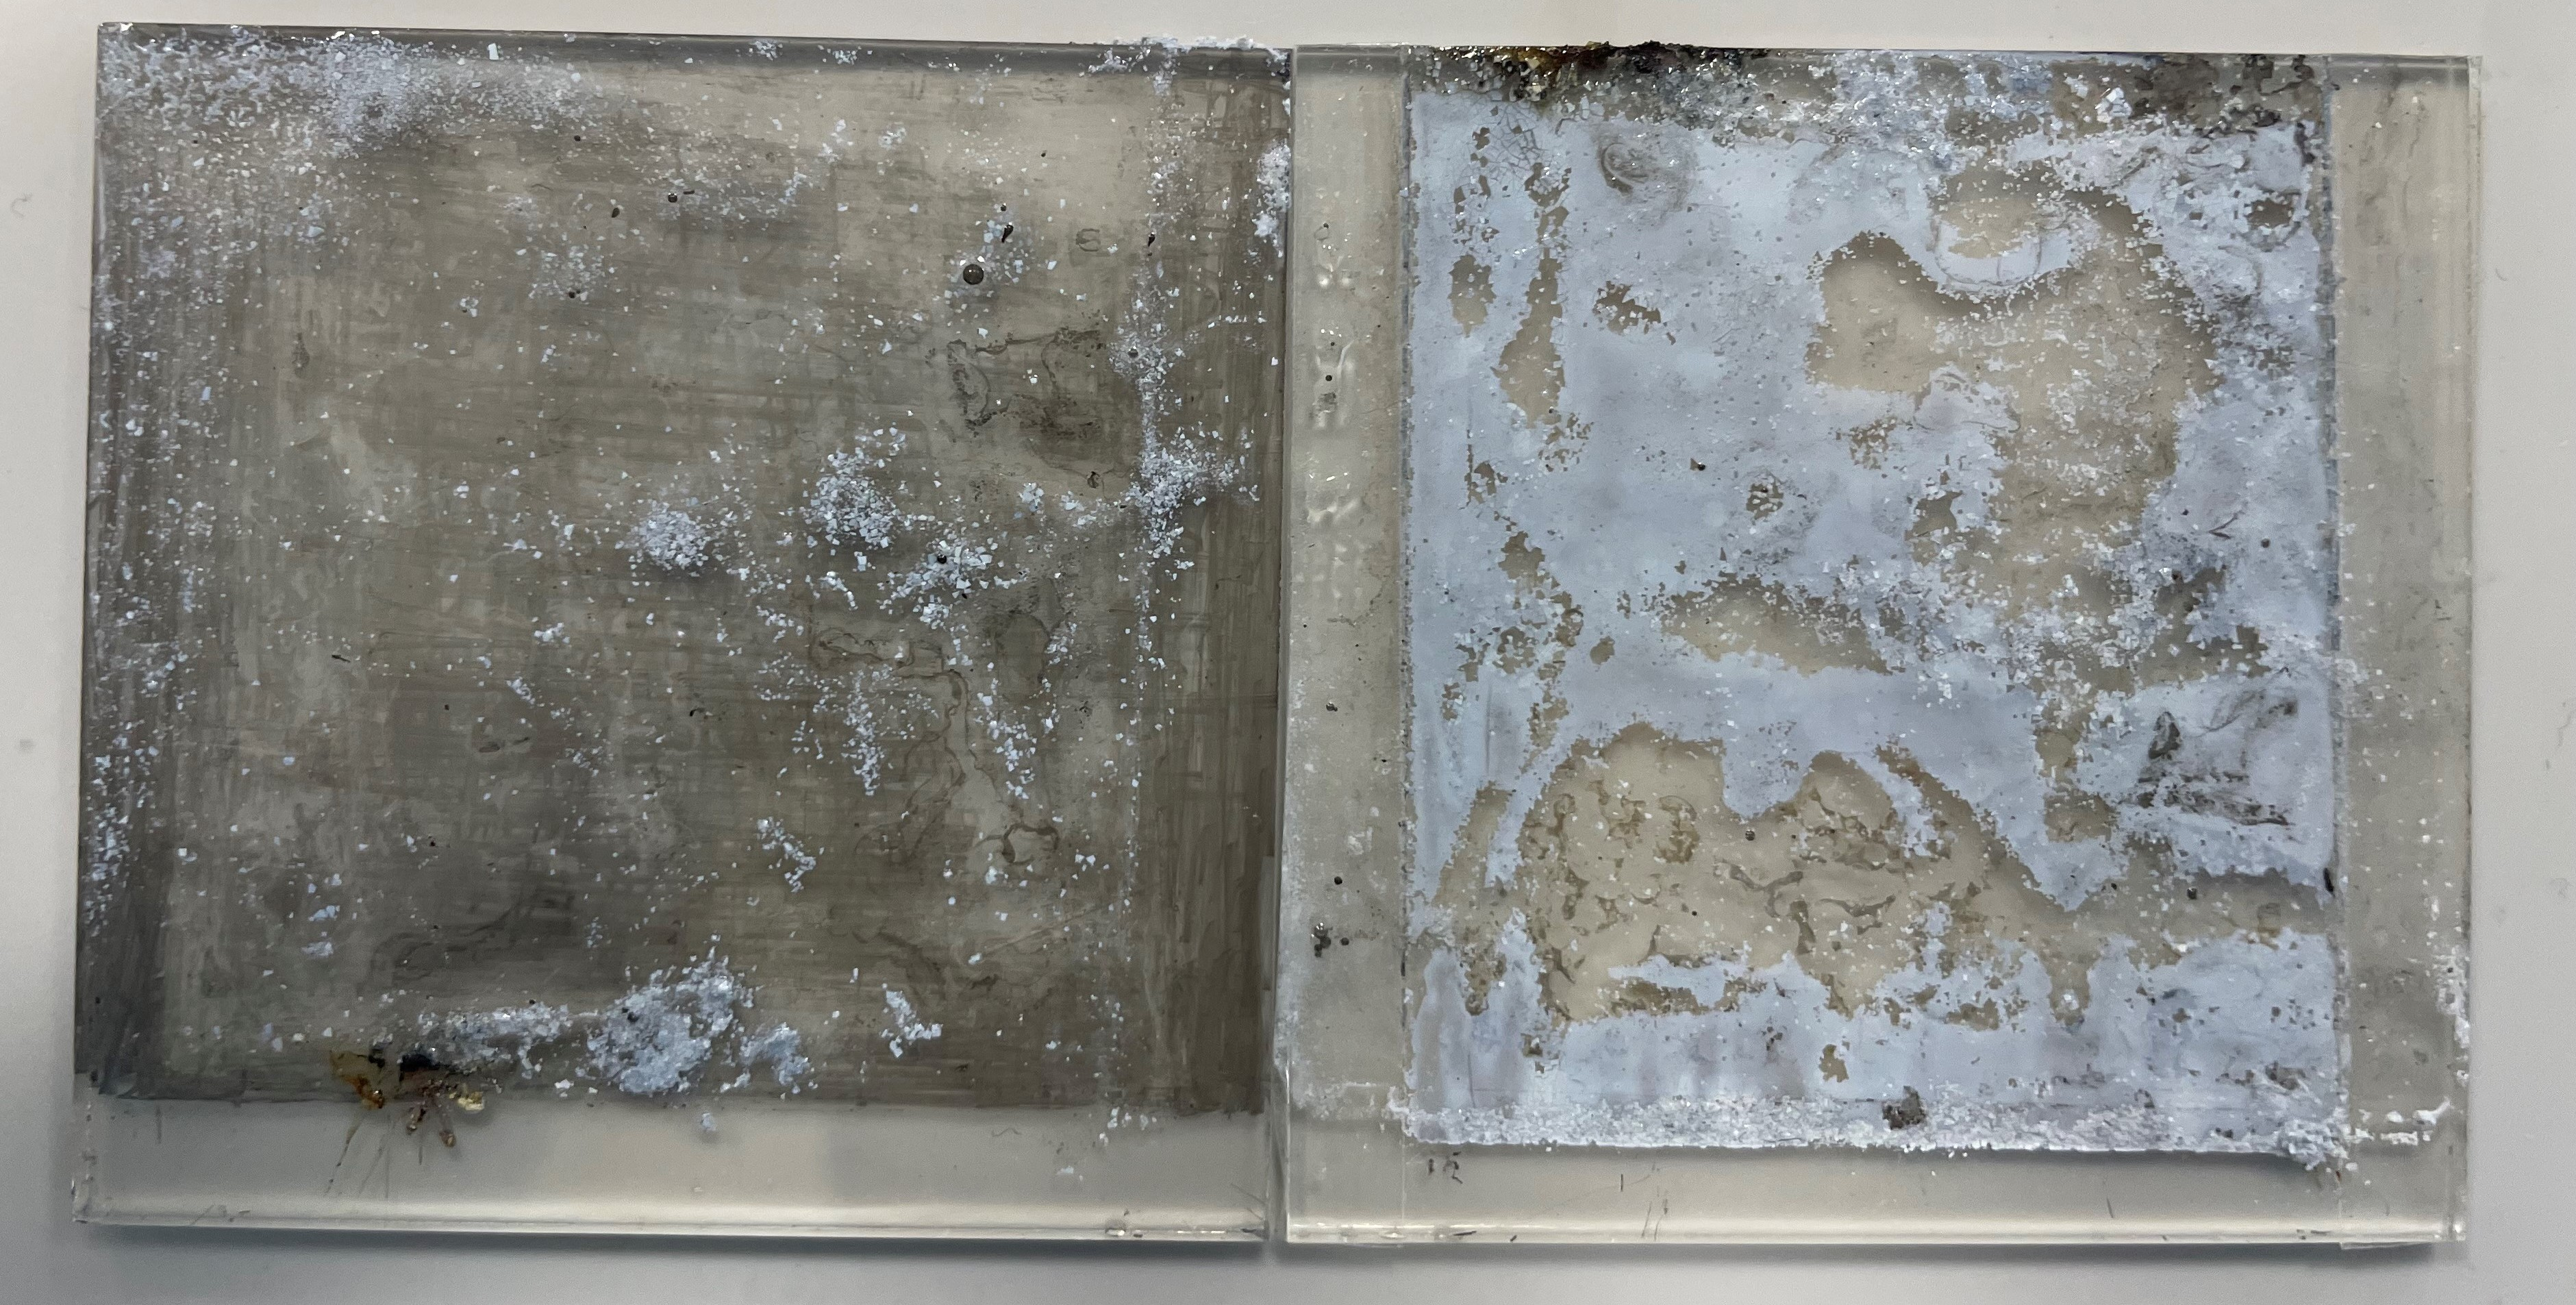
\includegraphics[width=0.388\textwidth]{degraded_cathode}}
\subfloat[]{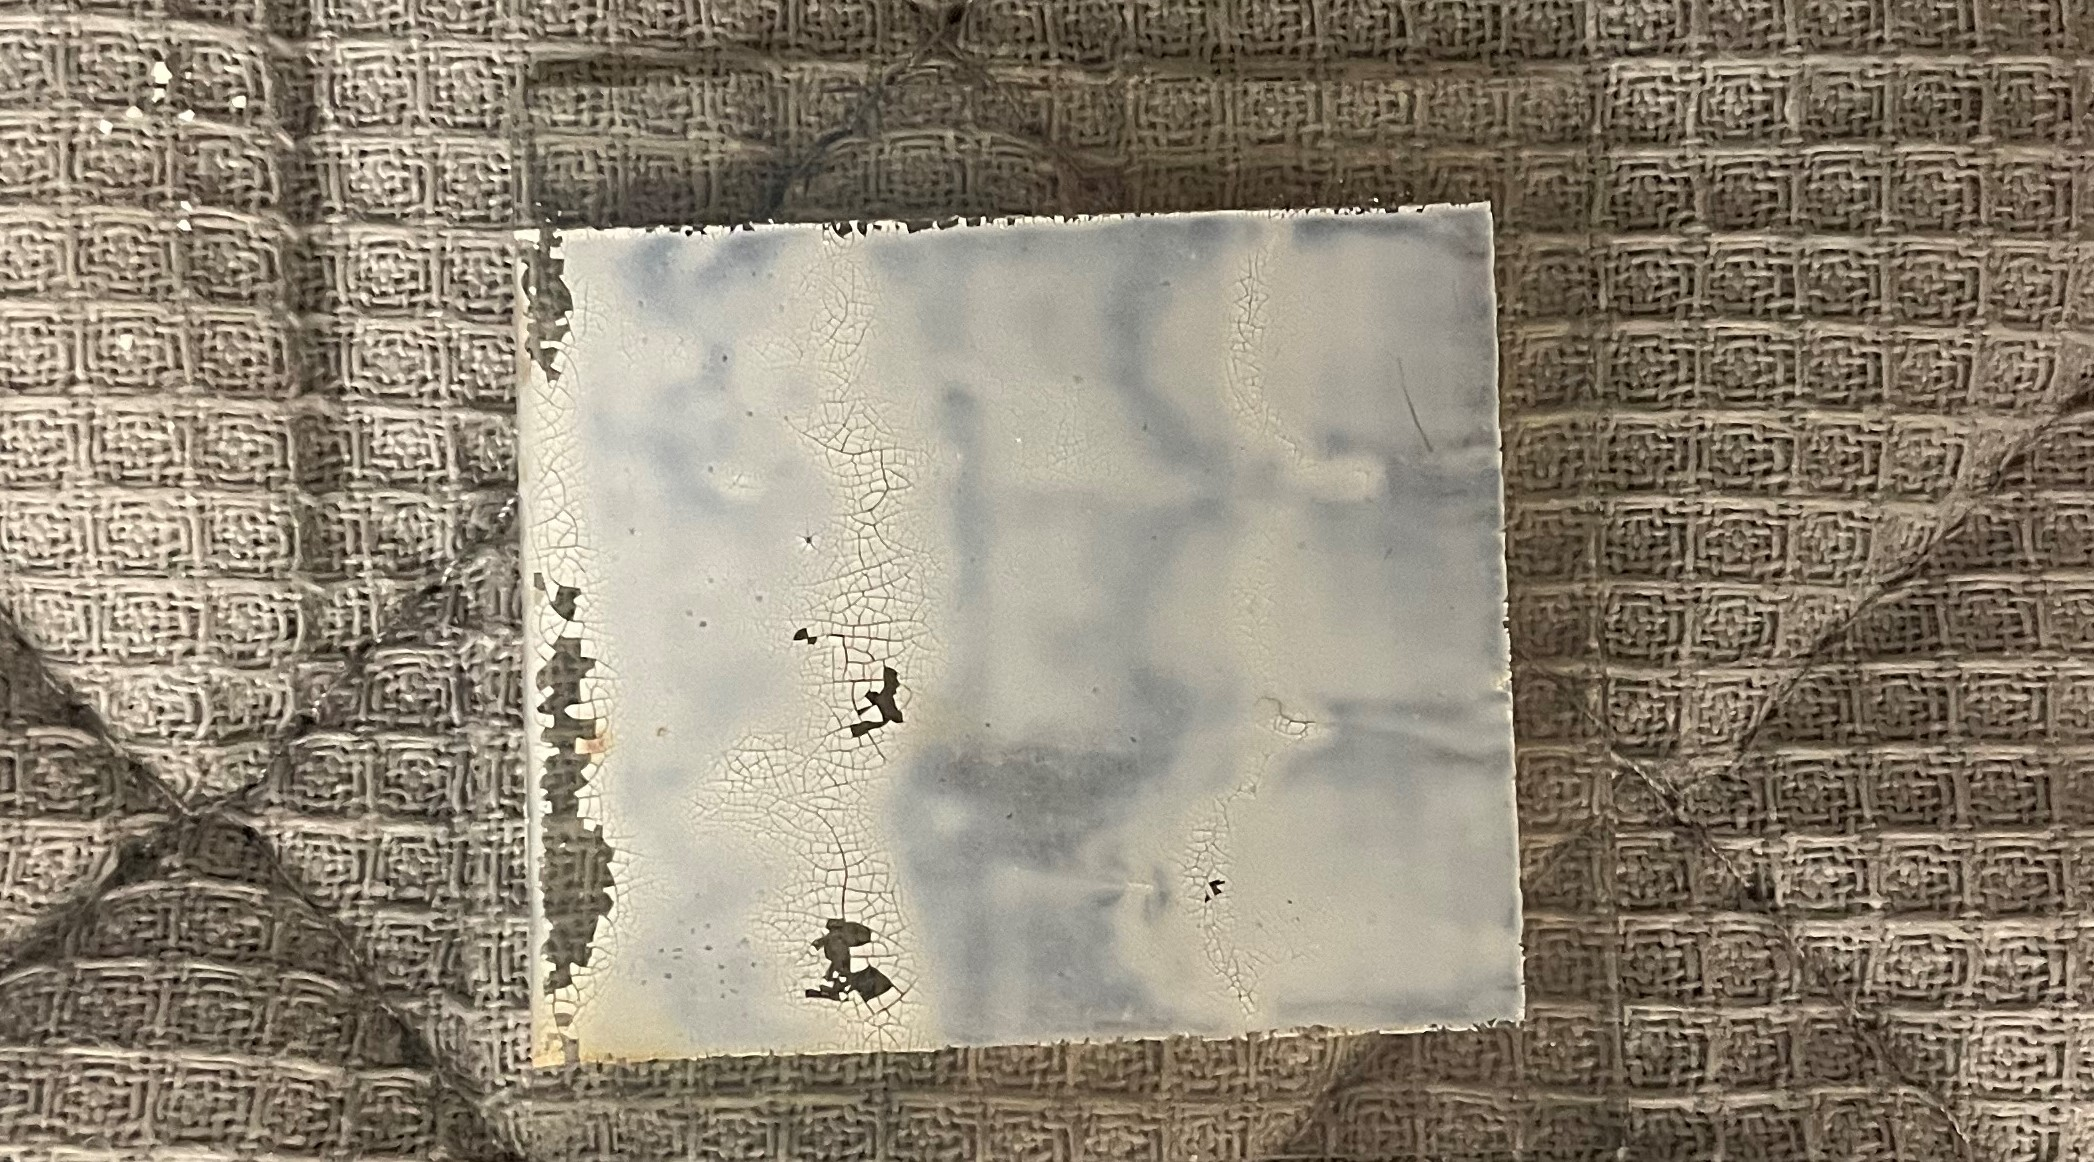
\includegraphics[width=0.353\textwidth]{cracked_cathode}}
\caption{(a): The soot anode during use. (b): A degraded cathode. (c): A too thick, cracked cathode.}
\label{fig:degradedelectrodes}
\end{figure}

\begin{figure}[ht!]
\centering
\subfloat[]{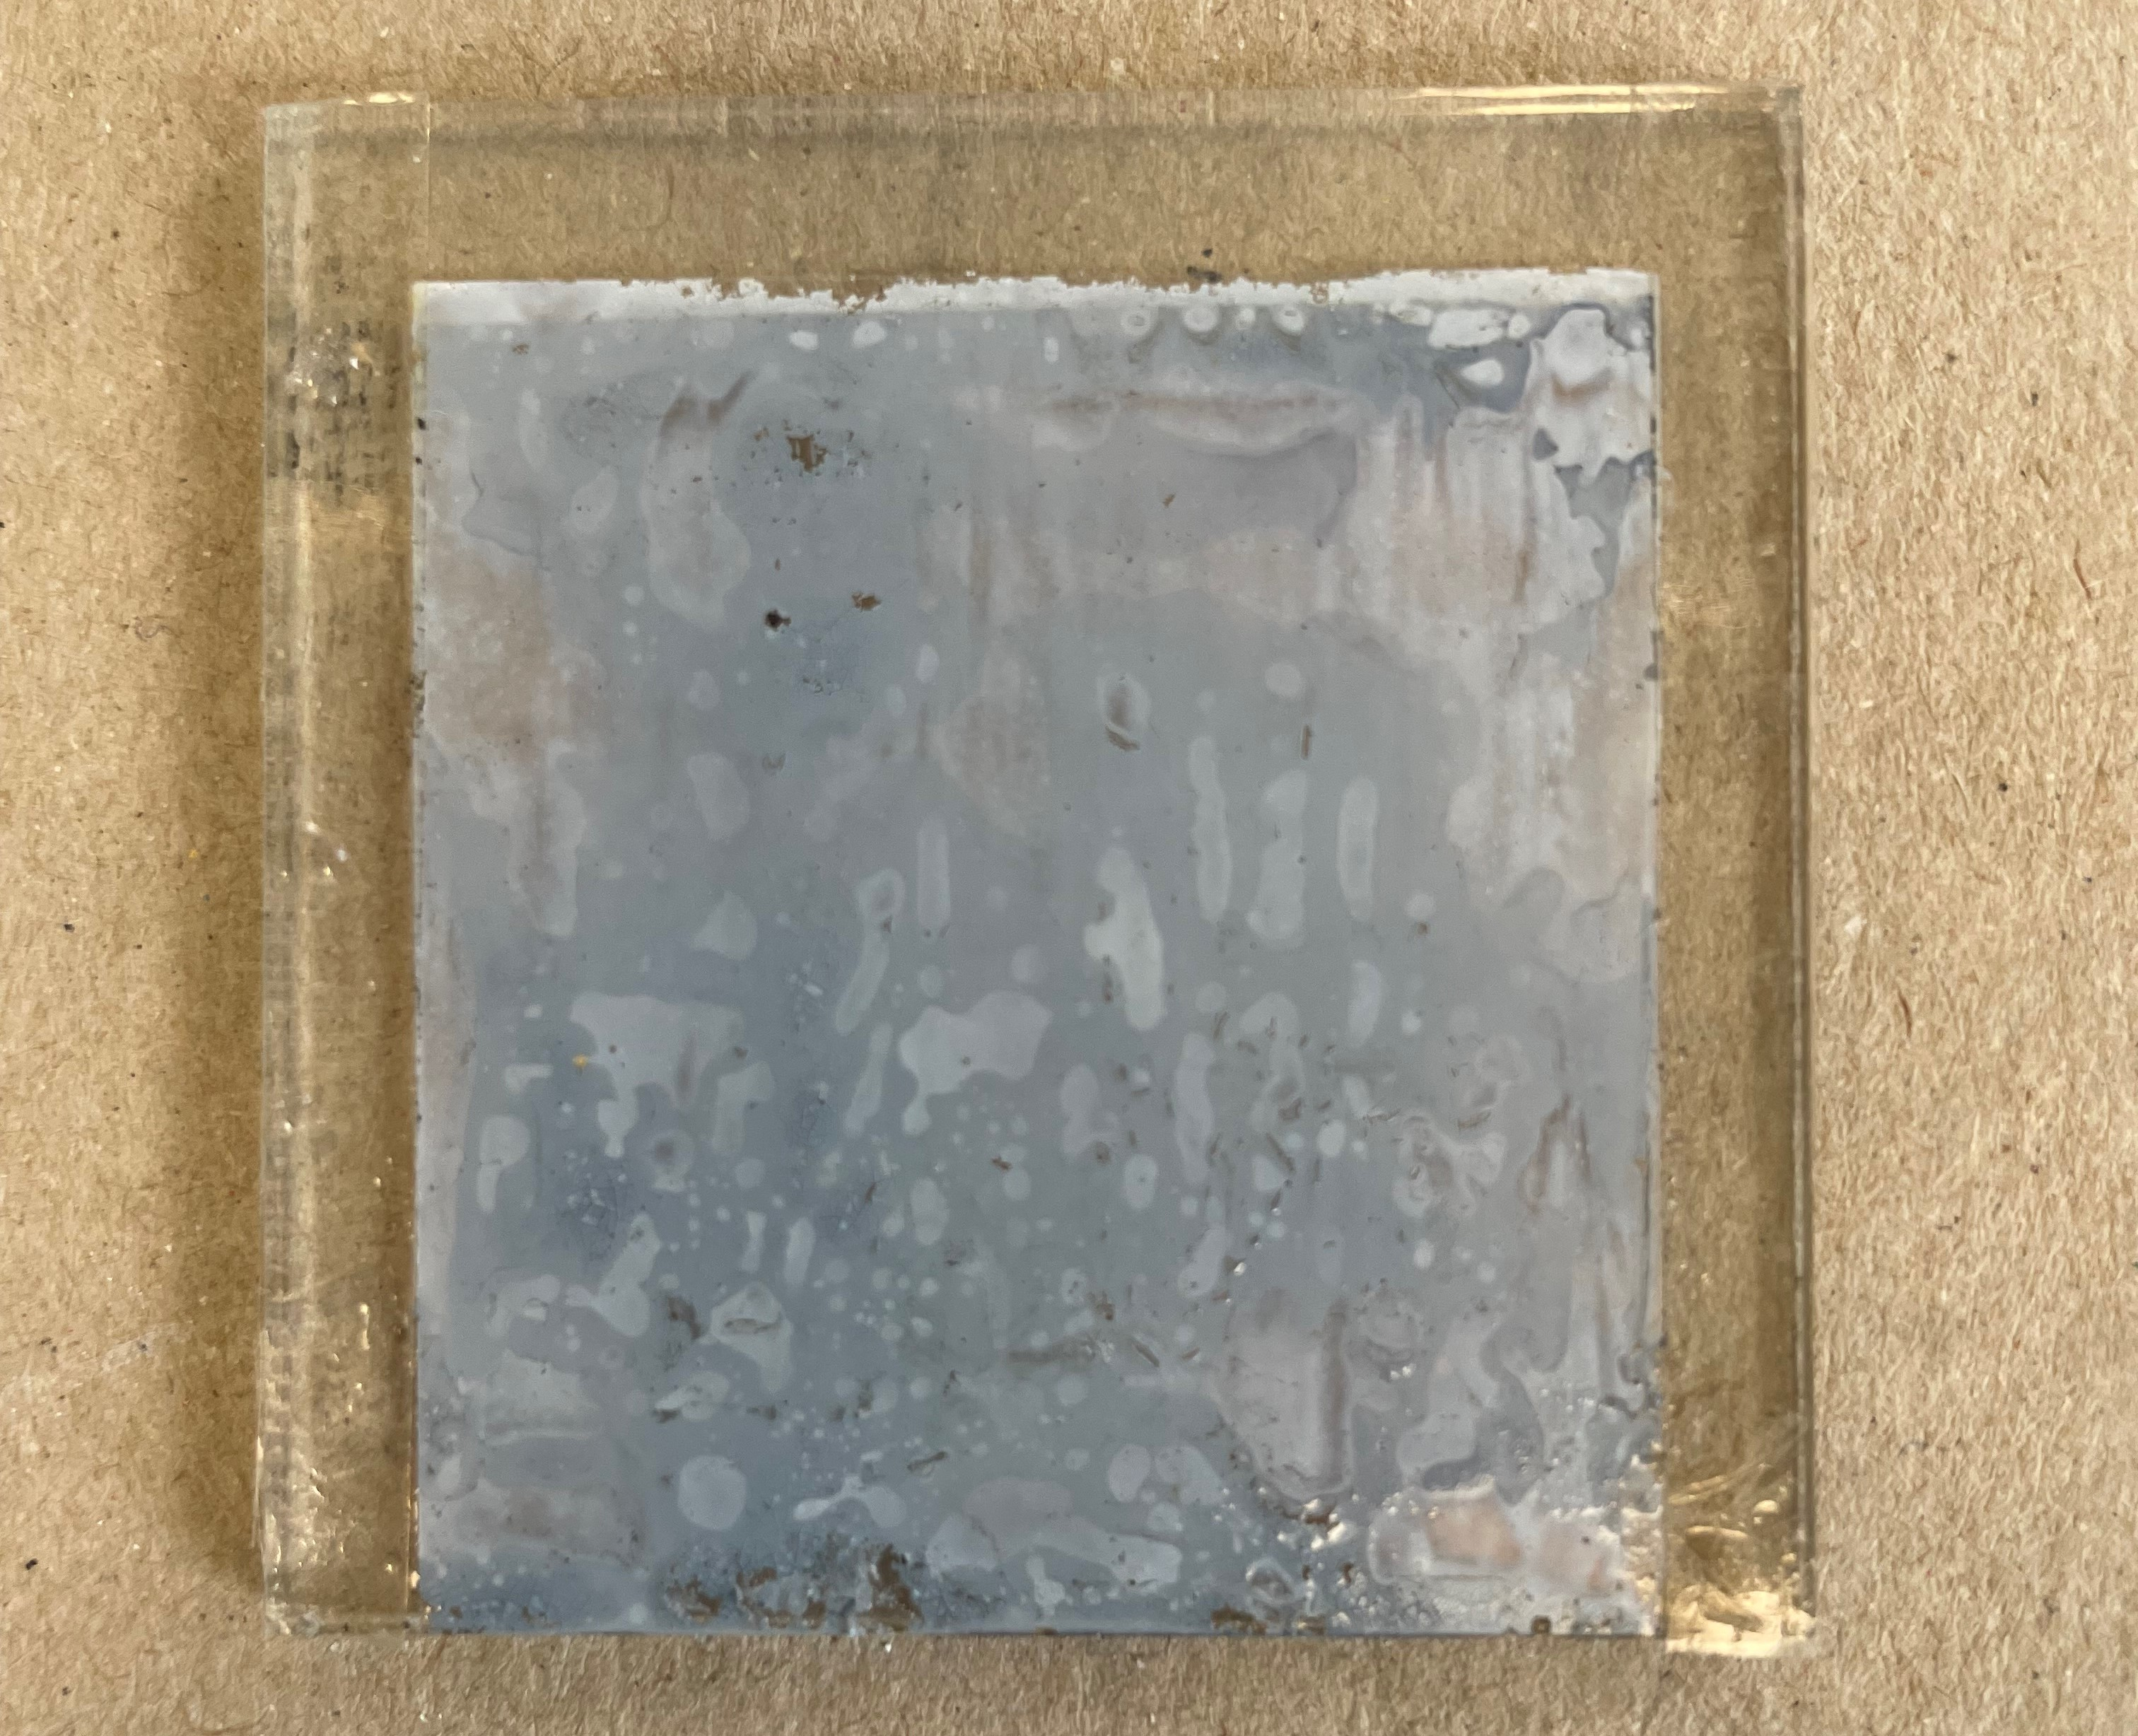
\includegraphics[width=0.443\textwidth]{charged_thick_cathode}}
\subfloat[]{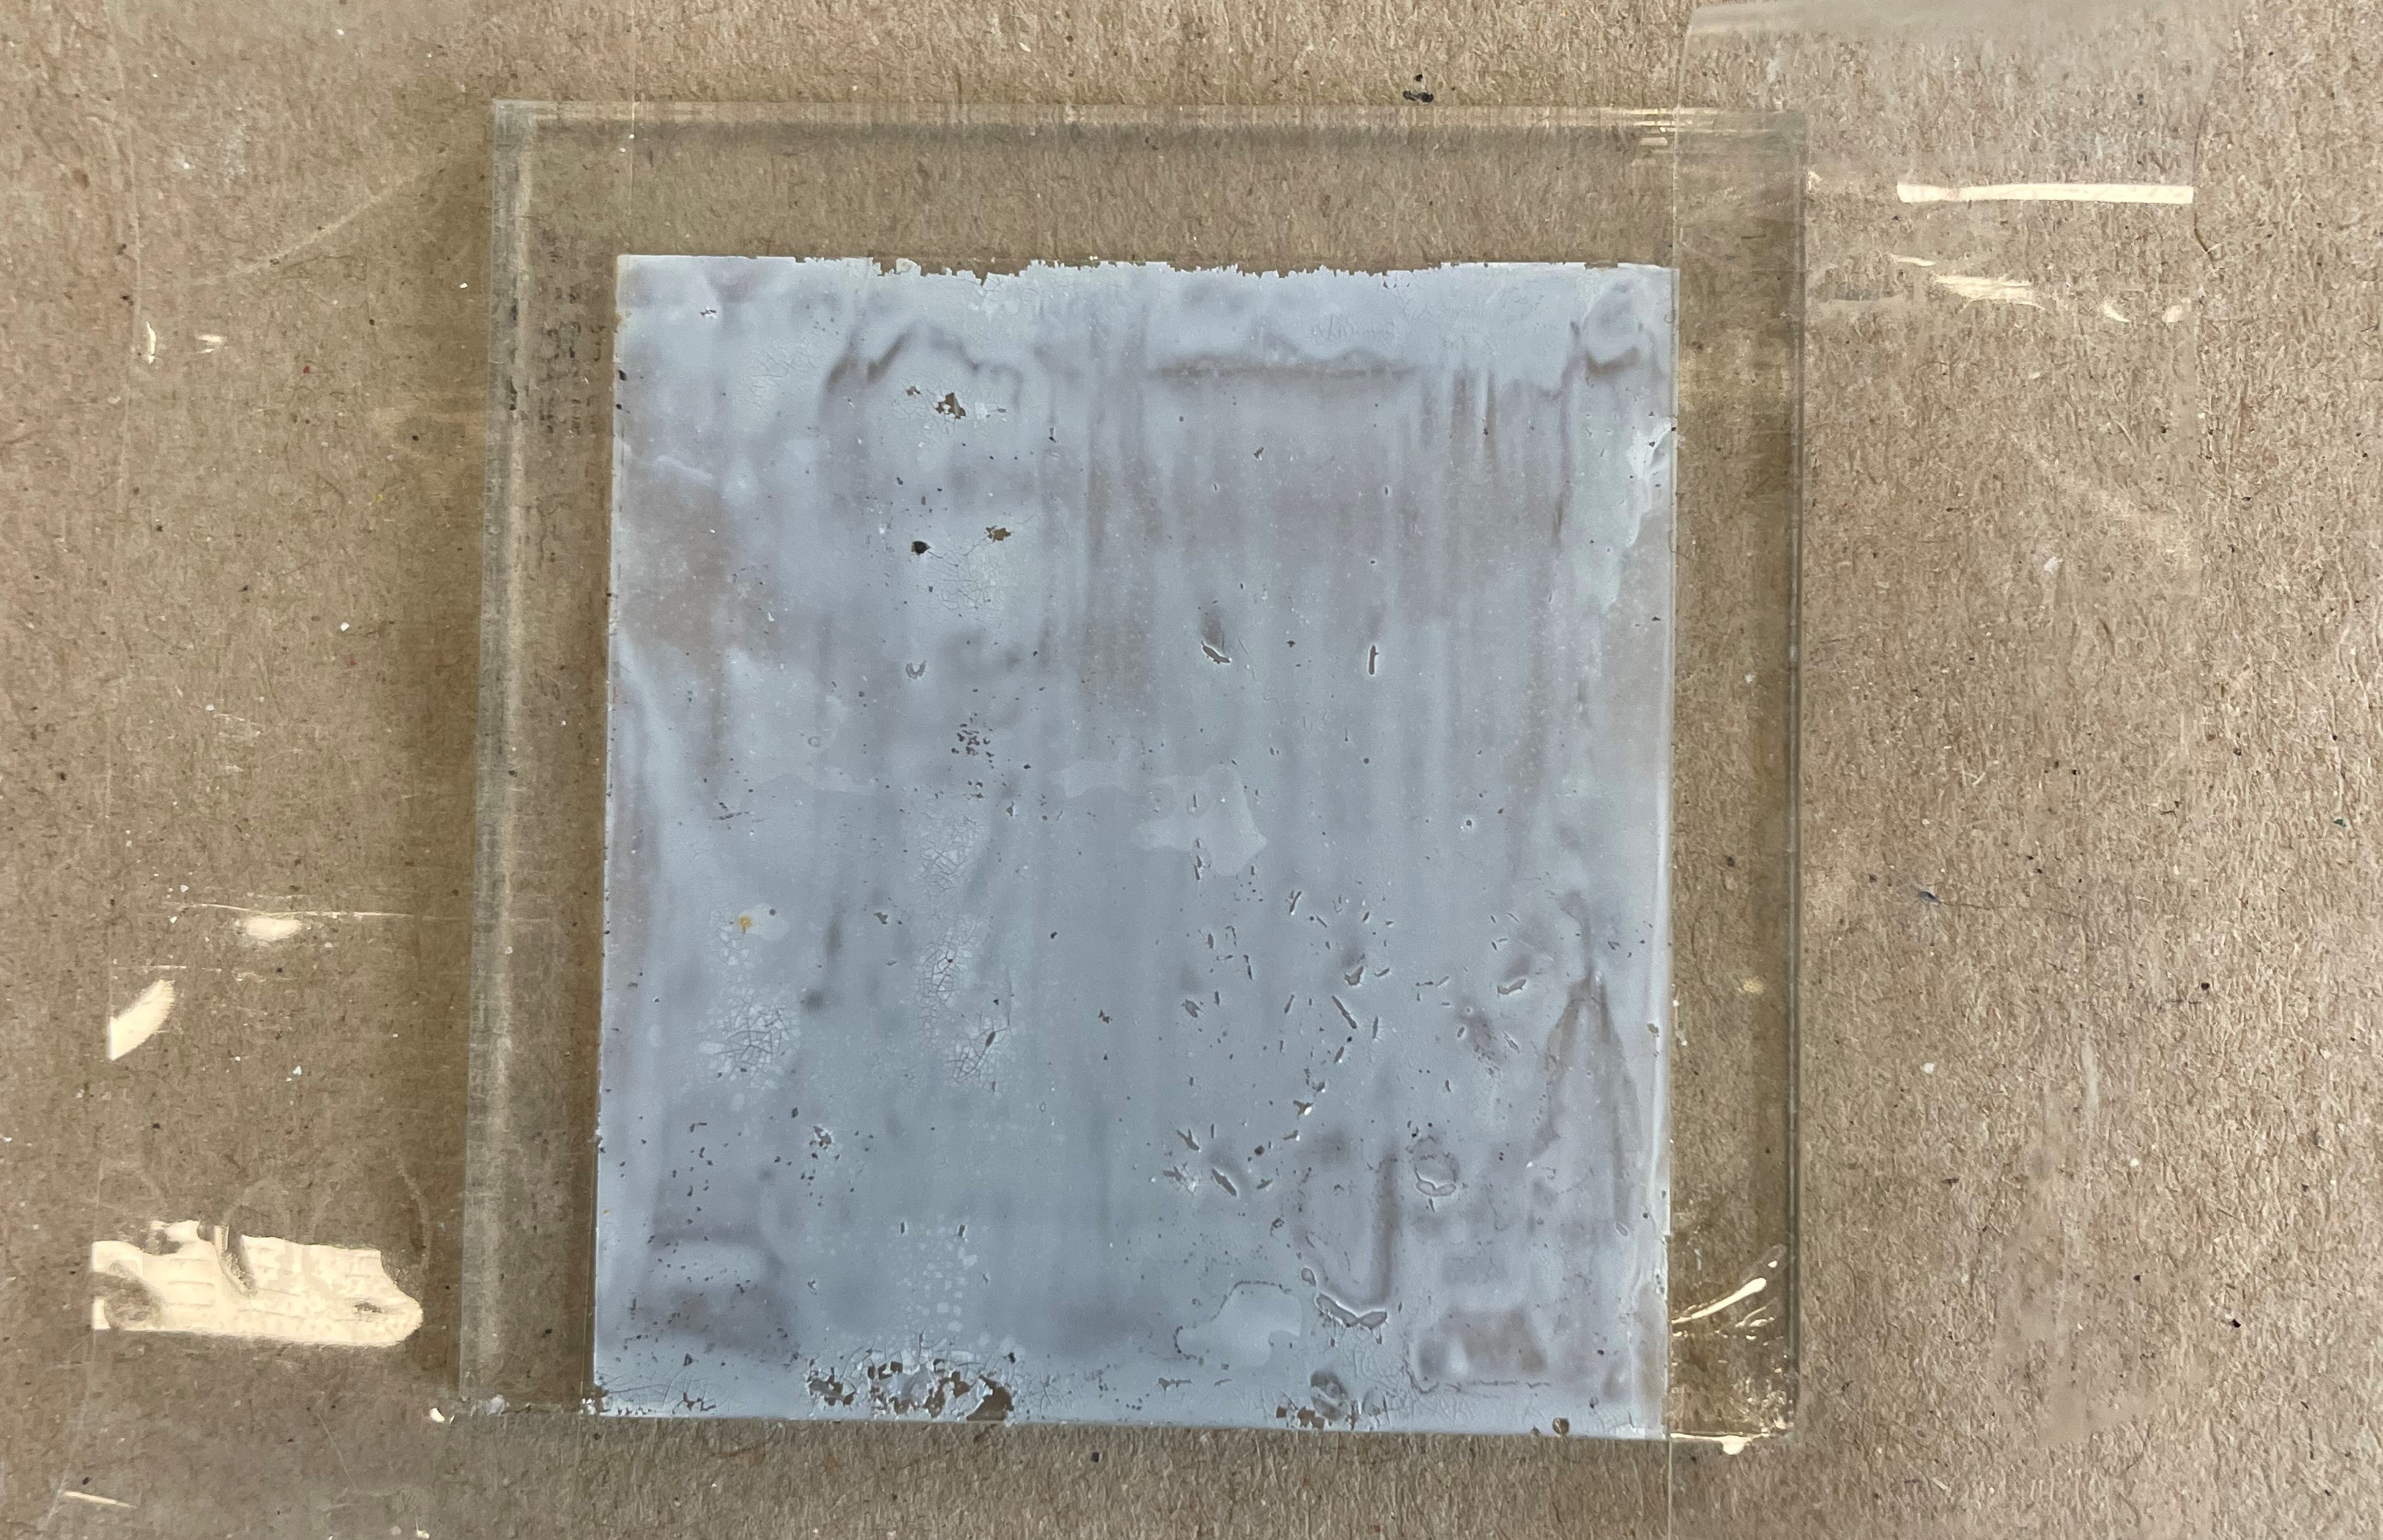
\includegraphics[width=0.557\textwidth]{charged_thin_cathode}}
\caption{(a): A charged, thick-layered cathode. (b): A charged, thin-layered cathode.}
\label{fig:chargedchathodes}
\end{figure}

\newpage
    
As shown in Fig. \ref{fig:anodecathodepairing}, a thick titanium-dioxide layer effectively outperforms a thinner layer both in terms of the charged to discharged voltage difference and the peak discharge current.
The thin-layered cathode achieves a charged to discharged difference of $\Delta_{\text{thin}} = \SI{0.1}{\V} - \SI{0.025}{\V} = \SI{0.075}{\V}$ compared to the $\Delta_{\text{thick}} = \SI{0.5}{\V} - \SI{0.025}{\V} = \SI{0.475}{\V}$ charged to discharged delta presented by the thick-layered cathode.

In terms of peak discharge current, the thick-layered cathode outperforms the thin-layered cathode by a factor of four. However, as visible in Fig. \ref{fig:degradedelectrodes} (c) a thicker layer of titanium-dioxide is prone to cracks and disconnect from the FTO current collector. This leads to faster cathode degradation, shown in Fig. \ref{fig:degradedelectrodes} (b). After just a few discharge cycles, a large part of the titanium-dioxide coating has fallen off, and the cathode is burnt. 
However, a thinner titanium-dioxide layer offers less sodium-ion storage. This can be seen through the difference in color intensity between a charged, thin titanium-dioxide coating and a charged, thick coating in Fig. \ref{fig:chargedchathodes}. The thick-layered cathode (a) is visibly more blue than the thin-layered cathode (b), which indicates a higher quantity  of intercalated sodium-ions.
Furthermore, as visible in Figs. \ref{fig:anodecathodepairing} and \ref{fig:degradedelectrodes} (a), soot as an anode substance is not compatible with a water-based electrolyte, as it suspends in the aqueous solution and detaches from the FTO glass slide.

\newpage

\begin{figure}[ht!]
\centering
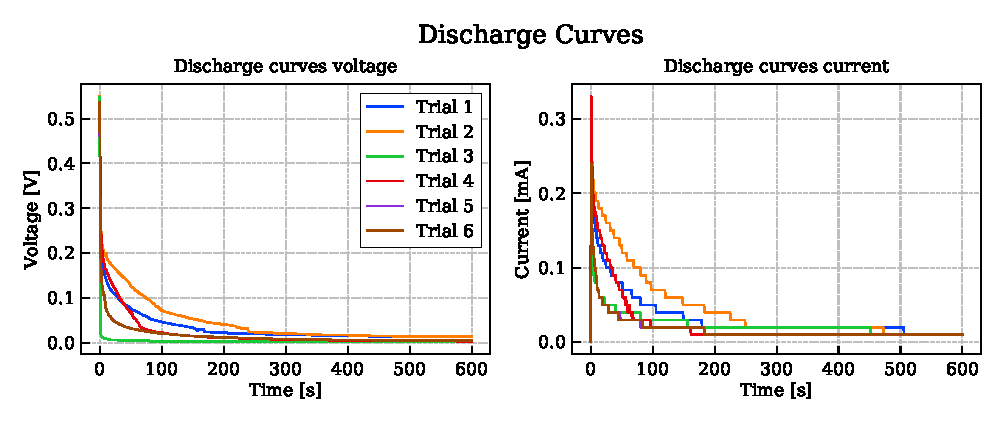
\includegraphics[width=\textwidth]{images/dischargefig.eps}
\caption{The voltage and current discharge curves of two different batteries over two different loads with varying charge times.}
\label{fig:dischargecurves}
\end{figure}

\begin{table}[ht!]
\centering
\begin{tabular}{c||c|c}
\bfseries Trial & \bfseries Charge time & \bfseries Resistance \\
\hline\hline
Trial 1 & \multirow{2}{*}{\SI{10}{\minute}} &\SI{1e3}{\ohm} \\
\cline{1-1}\cline{3-3}
Trial 2 &&\SI{1e2}{\ohm} \\
\hline
Trial 3 & \SI{20}{\minute} &\SI{1e3}{\ohm} \\
\hline
Trial 4 & \multirow{2}{*}{\SI{10}{\minute}} &\SI{1e3}{\ohm} \\
\cline{1-1}\cline{3-3}
Trial 5 &&\SI{1e2}{\ohm} \\
\hline
Trial 6 & \SI{20}{\minute} &\SI{1e3}{\ohm} \\
\hline
\end{tabular}
\caption{Trial descriptions.}
\label{tab:trialdescriptions}
\end{table}

The discharge curves obtained do not resemble those produced by commercially available batteries, since no rated voltage is held over a longer period \cite{Panasonic2018}. Instead, both the voltage and current discharge curves decline rapidly. 
As can be expected through the relationship between current, voltage and resistance: $\mathrm{U}=\mathrm{R} \cdot \mathrm{I}$ and as visible through the grey and green curves in Fig. \ref{fig:dischargecurves}, a lower load resistance of \SI{1e2}{\ohm} compared to \SI{1e3}{\ohm} results in a lower voltage curve overall.
Counterintuitively, the corresponding current curves similarly dropped overall, instead of increasing.
Furthermore, a longer charging period seems to impact battery 1, but not battery 2, as displayed by the generally higher orange curve compared to the more average brown curve in Fig. \ref{fig:dischargecurves}.

\newpage

\subsection{Data Analysis}
The capacity of the batteries can be determined by integrating the current discharge curves and calculating the area under the curve, as described in equation \ref{eq:capacityequation} and demonstrated in equation \ref{eq:capacityexample}. The integral was numerically approximated using the midpoint rule and a discretization time-step $\Delta t = t_i - t_{i-1} = \SI{1}{\second}$\cite{Kammer2019}.

\begin{align}\label{eq:capacityexample}
    Q &= \int_0^T I \cdot t \cdot d t \approx \sum_{i=1}^{T} \frac{I_i + I_{i-1}}{2} \cdot (t_{i}-t_{i-1}) \Rightarrow Q = \SI{1.92e-2}{\coulomb} \quad \text{duration } T = \SI{600}{\second}\\
    Q &= \SI{5.33e-3}{\mA\hour}
\end{align}


Additionally , the average power output can be calculated, by multiplying the average current by the average voltage. As mentioned in equation \ref{eq:powerequation} and demonstrated in equation \ref{eq:powerexample}.

\begin{align}\label{eq:powerexample}
    I_\text{average} &= \frac{1}{n}\sum_{i=1}^{n} I_i \Rightarrow I_\text{average} = \SI{3.19e-5}{\ampere} \quad \text{duration } n = \SI{600}{\second}\\
    U_\text{average} &= \frac{1}{n}\sum_{i=1}^{n} U_i \Rightarrow U_\text{average} = \SI{3.14e-3}{\volt} \quad \text{duration } n = \SI{600}{\second}\\
    P_\text{average} &= I_{\text{average}} \cdot  U_\text{average} = \SI{3.2e-5}{\ampere} \cdot \SI{3.14e-3}{\volt} = \SI{1.00e-3}{\watt}\\
\end{align}

All calculations were done in Microsoft Excel and can be verified online\cite{Hoffman2022}.

\begin{table*}[!ht]
\renewcommand{\arraystretch}{1.3}
\centering
\begin{tabular}{c |c |c||c|c}
\bfseries Trial & $T_\text{charge}$ [\unit{\min}] & Resistance [\unit{\ohm}] & $Q$ [\unit{\mA\hour}] & $P_\text{average}$ [\unit{\W}]\\
\hline\hline
\multirow{3}{*}{Battery 1}&\multirow{2}{*}{$10$}&\num{1e3}&\num{5.33e-3}&\num{1.00e-3}\\
\cline{3-5}
& &\num{1e2}&\num{3.89e-3}&\num{7.29e-5}\\
\cline{2-5}
&$20$&\num{1e3}&\num{7.33e-3}&\num{1.96e-3}\\\hline\hline
\multicolumn{3}{c||}{\bfseries Average}&\num{5.52e-3}&\num{1.01e-3}\\\hline\hline
\multirow{3}{*}{Battery 2}&\multirow{2}{*}{$10$}&\num{1e3}&\num{3.83e-3}&\num{4.75e-4}\\
\cline{3-5}
& &\num{1e2}&\num{2.85e-3}&\num{2.58e-4}\\
\cline{2-5}
&$20$&\num{1e3}&\num{2.85e-3}&\num{2.57e-4}\\\hline\hline
\multicolumn{3}{c||}{\bfseries Average}&\num{3.18e-3}&\num{3.30e-4}\\\hline
\end{tabular}
\caption{Capacity and power calculation results}
\label{table:results}
\end{table*}

